
\section[Speedup (Aside)]{Speedup (Aside)}
\label{sec:speedup}
\addcontentsline{toc}{section}{\thesection. Speedup (Aside)}

The main bottleneck of \pkg{cubfits} is at calls to \code{fitMultinom*()} or
\code{my.fitMultinom*()}. The reasons are that
\begin{itemize}
\item models assume conditional independent of amino acids, and
\item tedious to parallelize within \code{VGAM::vglm()} function.\footnote{
As long as number of sequences is not too large and summarized statistics is
used, there is no need to consider this approach. Although this can lead to
huge improvement of speedup, the cost may be too high that needs to rewrite
whole \code{vglm()} and reorganize data structures.
}
\end{itemize}
Fortunately, carefully utilize summarized data structures can avoid some
burdens and boost the MCMC computing a lot. For example, sorting by ORF's
names before MCMC may avoid subset a \code{data.frame} in some computing, and
further computing can be moved to \proglang{C} easily.

Further, \pkg{cubfits} consider three ways of parallel computations to
speedup computations, including
\code{parallel::mclapply()}, \code{pbdMPI::task.pull()}, and
\code{pbdMPI::pbdLapply()}. Note that only \pkg{pbdMPI} functions are tested
thoroughly in \pkg{cubfits} by default.


\subsection[mclapply]{mclapply}
\label{sec:mclapply}
\addcontentsline{toc}{subsection}{\thesubsection. mclapply}

The function \code{mclapply()}
is a default function in \pkg{parallel} and particularly useful for
multi-cores and shared memory machines, but only for Unix-like systems such
as Linux and Mac OS.
In Windows system, this function is the same as \code{lapply()} since
forking mechanism differs from Unix-like systems.
\code{mclapply()} is a parallel version of \code{lapply()}, and is
easy to migrate from \code{lapply()}. So, this is first basic way to
speedup \pkg{cubfits}.

We consider to split jobs (tasks) in the level of 20 amino acids since the
conditional independence. Even though, the computation bottleneck held by some
amino acids that have more synonymous codons than others, e.g. Leucine (Leu/L)
has 6 synonymous codons. This means that 20 jobs are not homogeneous and Leu
probably needs the longest computing in those \code{fitMultinom*()} calls.
Therefore, we consider to use the option \code{mc.preschedule = FALSE} set to
\code{mclapply()}, and limit the number of cores to 4 or 5. In such a way, we
gain the performance economically.

However, in the warning section of \code{mclapply()} help page, it says
{\it \_strongly discouraged\_} to use these functions in GUI or embedded
environments, ...
For small tests, \code{mclapply()} is working well and efficient
in \pkg{cubfits}. Normally, less sequences and shorter MCMC iterations.
\pkg{cubfits} did observe some crashes occasionally
when using \code{mclapply()} for longer runs of MCMC, such as in a
work flow.


\subsection[task.pull]{task.pull}
\label{sec:task.pull}
\addcontentsline{toc}{subsection}{\thesubsection. task.pull}

If GUI or embedded environments were not the main targets, then a stable way
to speedup \pkg{cubfits} would be an idea way to aim for.
\pkg{pbdMPI} is designed in single program multiple data (SPMD) framework,
and is a simpler approach to parallelize codes.
Although only batch model is allowed in \pkg{pbdMPI},
one of the benefits is that it is not limited in multi-cores and
shared memory machines, and can be applied on most systems provided a
MPI library is installed.
See \citet{Chen2012pbdMPIvignette} for more details of installation of a
MPI library and \pkg{pbdMPI}.

The task pull is a simple way and has similar idea as
\code{mc.preschedule = FALSE} in \code{mclapply()} that gain
performance economically for non-homogeneous jobs.
\code{task.pull()} in \pkg{pbdMPI} is a simple implementation that can boost
\code{fitMultinom*()} functions, and has similar syntax as \code{mclapply()}.
Currently, \pkg{cubfits} is mainly tested under this way.


\subsection[pbdLapply]{pbdLapply}
\label{sec:pbdLapply}
\addcontentsline{toc}{subsection}{\thesubsection. pbdLapply}

For some cases, task pull is not economic nor efficient. For example, in
\pkg{cubfits} needs to initial expected expression level of each sequences
via a call to \code{estimatePhiAll*()}. On average, this is a pretty much
spending the same computation on all sequences. Therefore, task pull on 5,000
sequences may not a good idea since extra 5,000 calls for requesting unfinished
sequences are unavoidable in the task pull way.

The function \code{pbdLapply()} is similar to set \code{mc.preschedule = TRUE}
in \code{mclapply()}. The 5,000 sequences are divided by number of cores equally
likely and processed by each core simultaneously. In such a way, there is no
call for requesting sequences. Ideally, a good choice of number of cores
is related to number of sequences. In general, it needs to be tuned with a
few empirical runs.


\subsection[Performance]{Performance}
\label{sec:performance}
\addcontentsline{toc}{subsection}{\thesubsection. Performance}

Three different ways (\code{mclapply()}, \code{task.pull()}, and
\code{task.pull()}) are tested on Yeast genome which has about 5346 genes
and corresponding gene expression. Average run time of 200 iterations of
\code{cubfits()} are recorded in different number of cores. Then, the
speedup of parallelization is defined as each run time of given cores divides
the run time of one core of \code{mclapply()}.

Figure~\ref{fig:speedup} shows \code{task.pull()} is the best approach
although it needs one more core for task management. There is no best
choice for number of cores, but seven cores of \code{task.pull()} is pretty
much reach a bottleneck. The performance degradation of eight cores
of \code{pbdLapply()} is due to the unbalance pre-assignment of amino acid,
e.g. Leu and Arg are probably assigned to the same core.
The performance of \code{mclapply()} is surprisingly not well which may be
due to memory copying between forking mechanism and
\code{mc.preschedule = FALSE}.

\begin{figure}[ht]
\centering
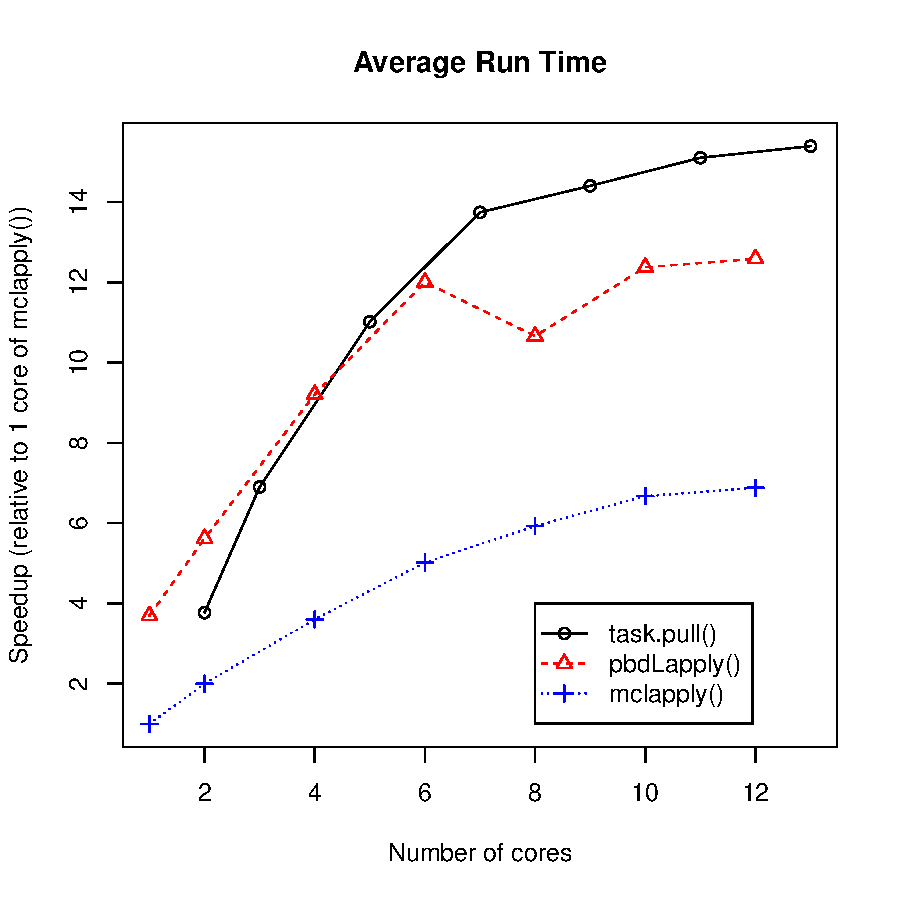
\includegraphics[width=4in]{cubfits-include/figure/avg_run_time}
\caption{Speedup of three different parallelizations.}
\label{fig:speedup}
\end{figure}
